\documentclass{beamer}

\usepackage{graphicx}
\usepackage[sfdefault,light]{FiraSans}
%\usefonttheme{serif} 
\usepackage[british]{datetime2}
\usetheme{default}
\setbeamertemplate{navigation symbols}{} % No navigation symbols
\setbeamercolor{alerted text}{fg=blue!80!green!159!}
\setbeamercolor{frame title}{fg=blue!80!green!159!}
\setbeamercolor{title}{fg=blue!80!green!159!}
\setbeamercolor{subtitle}{fg=blue!80!green!159!}

\makeatletter
\setbeamertemplate{footline}
{
  \leavevmode%
  \hbox{%
  \begin{beamercolorbox}[wd=.15\paperwidth,ht=2.25ex,dp=1ex,center]{institute in head/foot}%
    \usebeamerfont{title in head/foot}%
    \raisebox{-0.15cm}{
\includegraphics[width=1cm]{logo_ntnu_u-slagord.pdf}}
  \end{beamercolorbox}%
  \begin{beamercolorbox}[wd=.6\paperwidth,ht=2.25ex,dp=1ex,center]{institute in head/foot}%
    \usebeamerfont{title in head/foot}%
    \insertsection
  \end{beamercolorbox}%
  \begin{beamercolorbox}[wd=.15\paperwidth,ht=2.25ex,dp=1ex,center]{institute in head/foot}%
    \usebeamerfont{title in head/foot}%
    \insertshortdate
  \end{beamercolorbox}%
  \begin{beamercolorbox}[wd=.1\paperwidth,ht=2.25ex,dp=1ex,right]{institute in head/foot}%
    \usebeamerfont{title in head/foot} 
    \insertframenumber{} / \inserttotalframenumber\hspace*{2ex} 
  \end{beamercolorbox}}%
}
\makeatother

%----------------------------------------------------------------------------------------
%	TITLE PAGE
%----------------------------------------------------------------------------------------

\title{POL2012: Theories and Models in Political Economy}
\subtitle{Institutionalism and Keynesian Economics}
% \date{\today}
\date{}
\author{Marius Swane Wishman}
\institute{Department of Sociology and Political Science}

\begin{document}

\begin{frame}[plain]
\titlepage % Print the title page as the first slide
\centering % Comment out if second logo

\includegraphics[width=5cm]{logo_ntnu_u-slagord.pdf}
%\hspace{0.5cm} 
\includegraphics[width=5cm]{logo_ntnu_u-slagord.pdf} % Second logo
\end{frame}


\section{Institutionalism} % Sections can be created in order to organize your presentation into discrete blocks, all sections and subsections are automatically printed in the table of contents as an overview of the talk
%------------------------------------------------

\begin{frame}{Historical context}
              \begin{figure}
                \includegraphics[width=\textwidth]{../img/robbers.jpg}
                \label{fig:robbers}
             \end{figure}{}
\end{frame}{}

\begin{frame}{What is Institutional Economics?} % Can be a bit difficult, less clear cut and fewer "heroes", more particularist theories/models
      \begin{itemize}[<+- | alert@+>]
        \item Critique of the reductionism of neo-classical PE
        \item Evolution not Equilibrium
        \item Institutions and Power
        \item Bringing the "Political" back into "Political Economy"
        \item Critique of Capitalism % Reform > Revolution
      \end{itemize}
\end{frame}{}

\section{Thorstein Veblen 1857-1929}

\begin{frame}{Theory of the Leisure class (1899)}
    \begin{figure}
        \centering
        
\includegraphics[width=\textwidth]{../img/gatsby.jpg}
        %\caption{"Look at all this utility!"}
    \end{figure}{}
\end{frame}

\section{John Kenneth Galbraith (1908-2006)}

\begin{frame}{Power}

\begin{figure}[htpb]
	\centering
	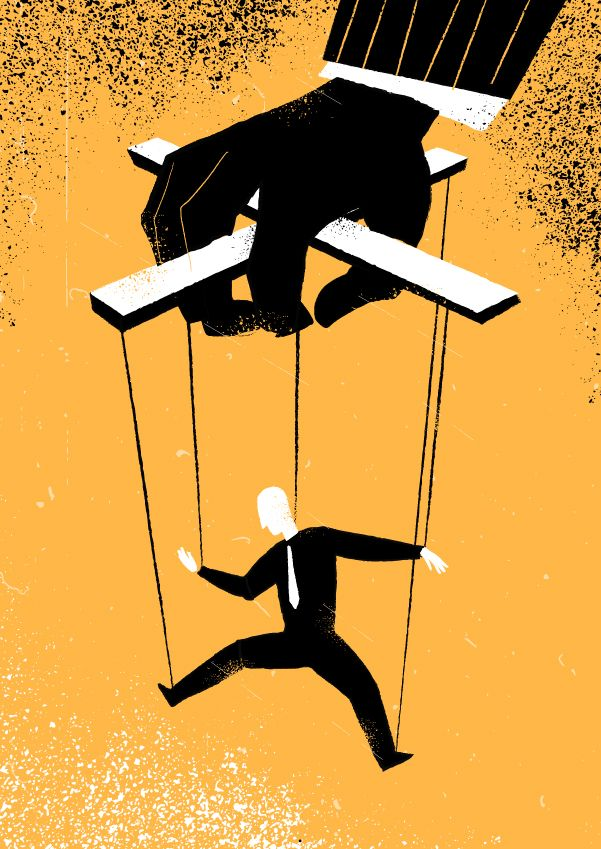
\includegraphics[width=0.5\textwidth]{../img/power.jpeg}
	\label{fig:power}
\end{figure}

\end{frame}{}

\begin{frame}{Technology}

\begin{figure}[htpb]
	\centering
	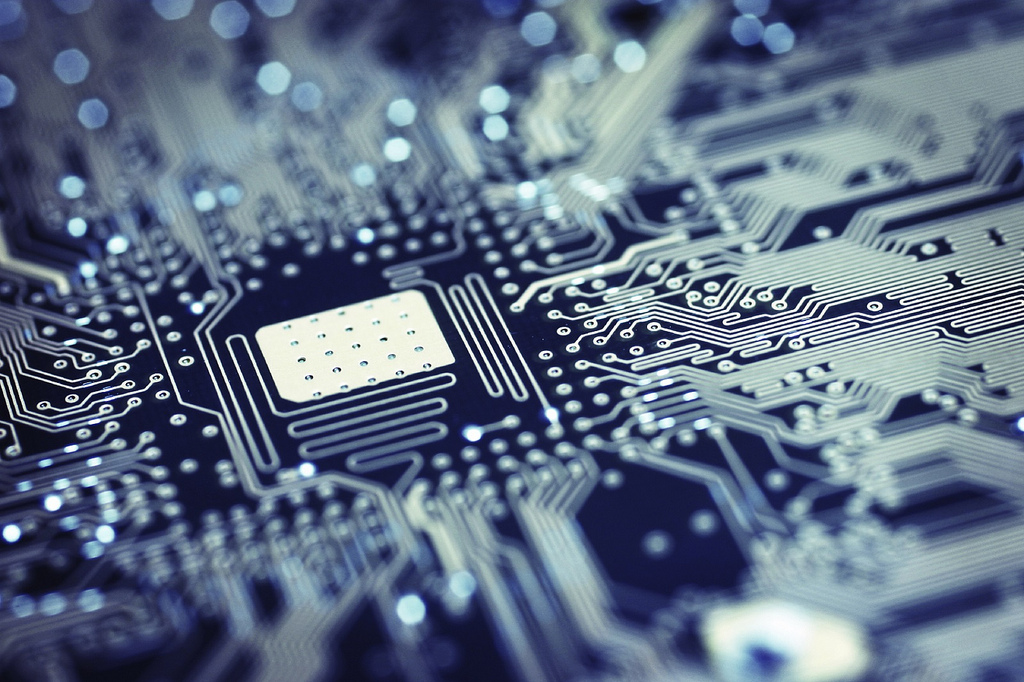
\includegraphics[width=0.8\textwidth]{../img/tech.jpg}
	\label{fig:technology}
\end{figure}

\end{frame}{}

\begin{frame}{The technostructure}

\begin{figure}[htpb]
	\centering
	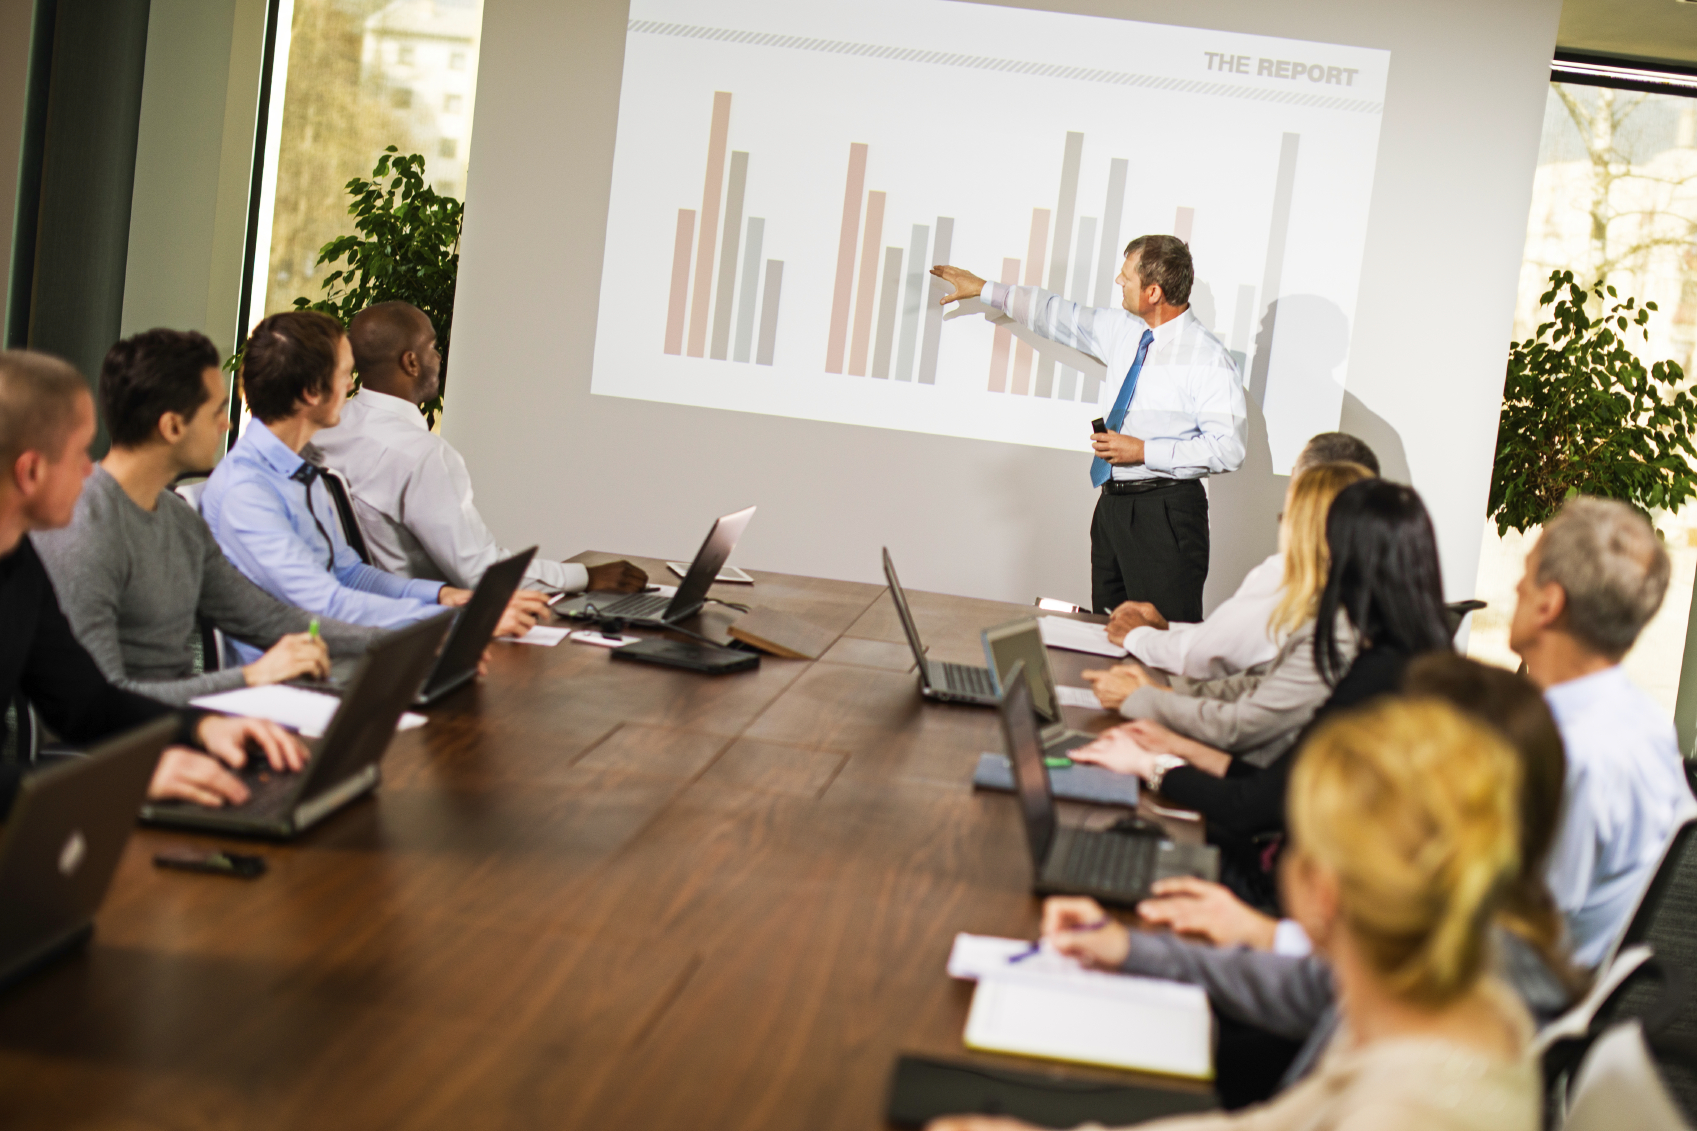
\includegraphics[width=0.8\textwidth]{../img/technostructure.jpg}
\end{figure}

\end{frame}

\begin{frame}{Rise of the Corporation}

	\begin{figure}[htpb]
		\centering
		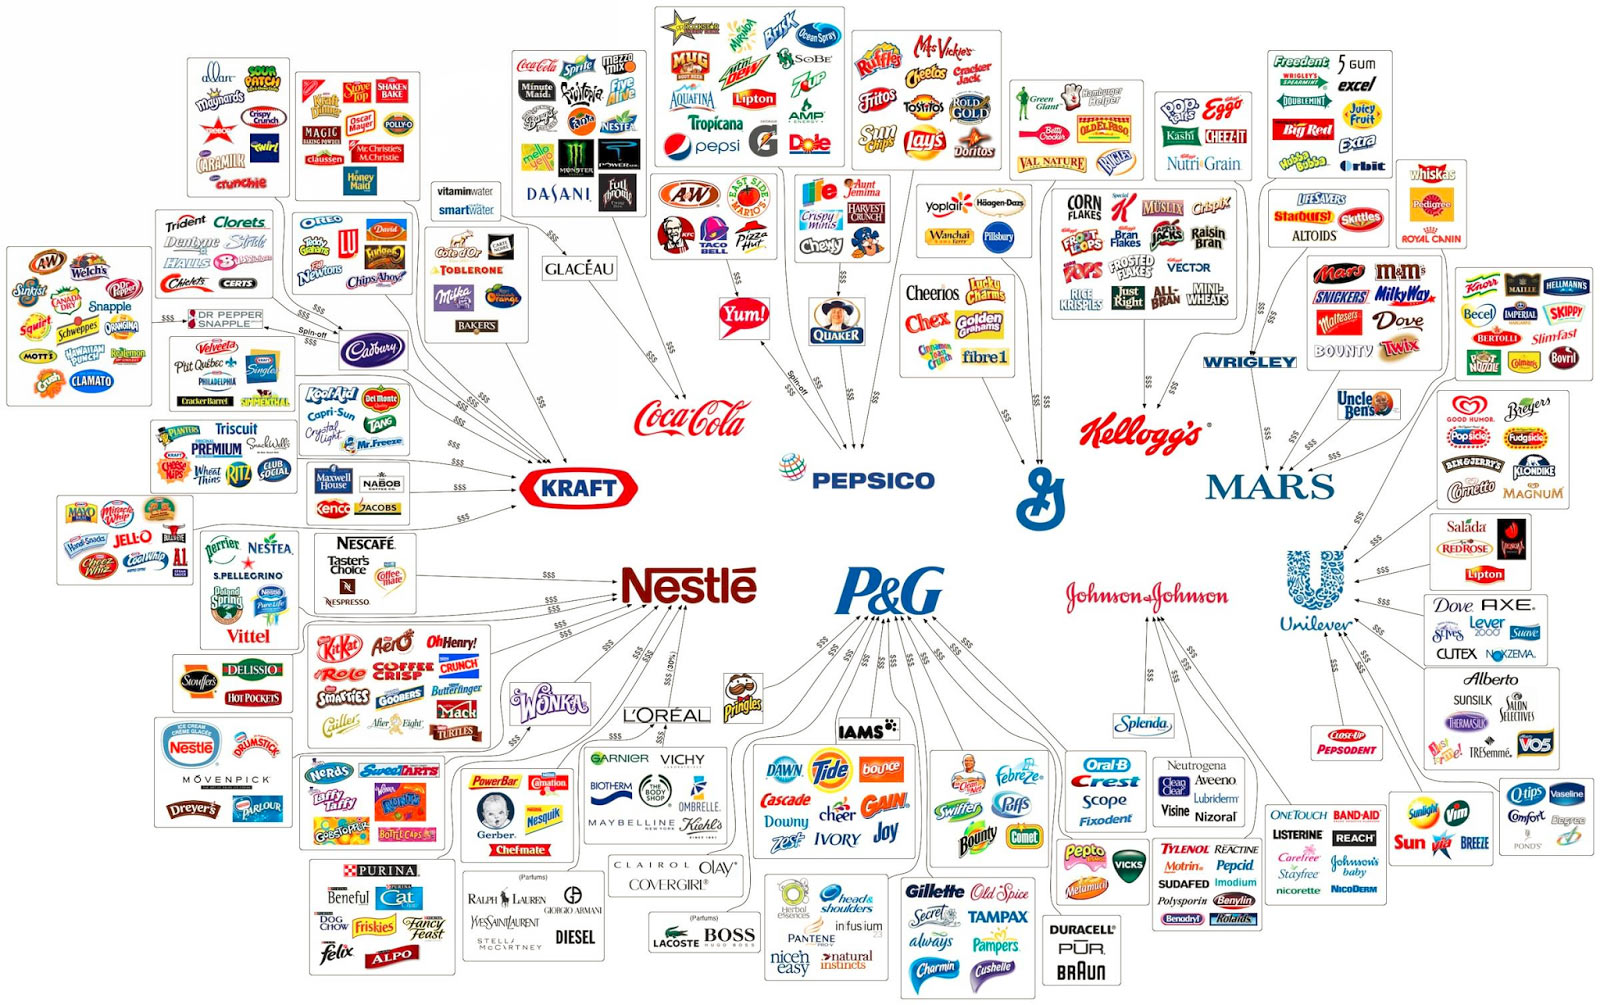
\includegraphics[width=0.8\linewidth]{../img/megacorp.jpg}
	\end{figure}

\end{frame}

\begin{frame}{Corporate Globalization} 
\begin{figure}
    \centering
    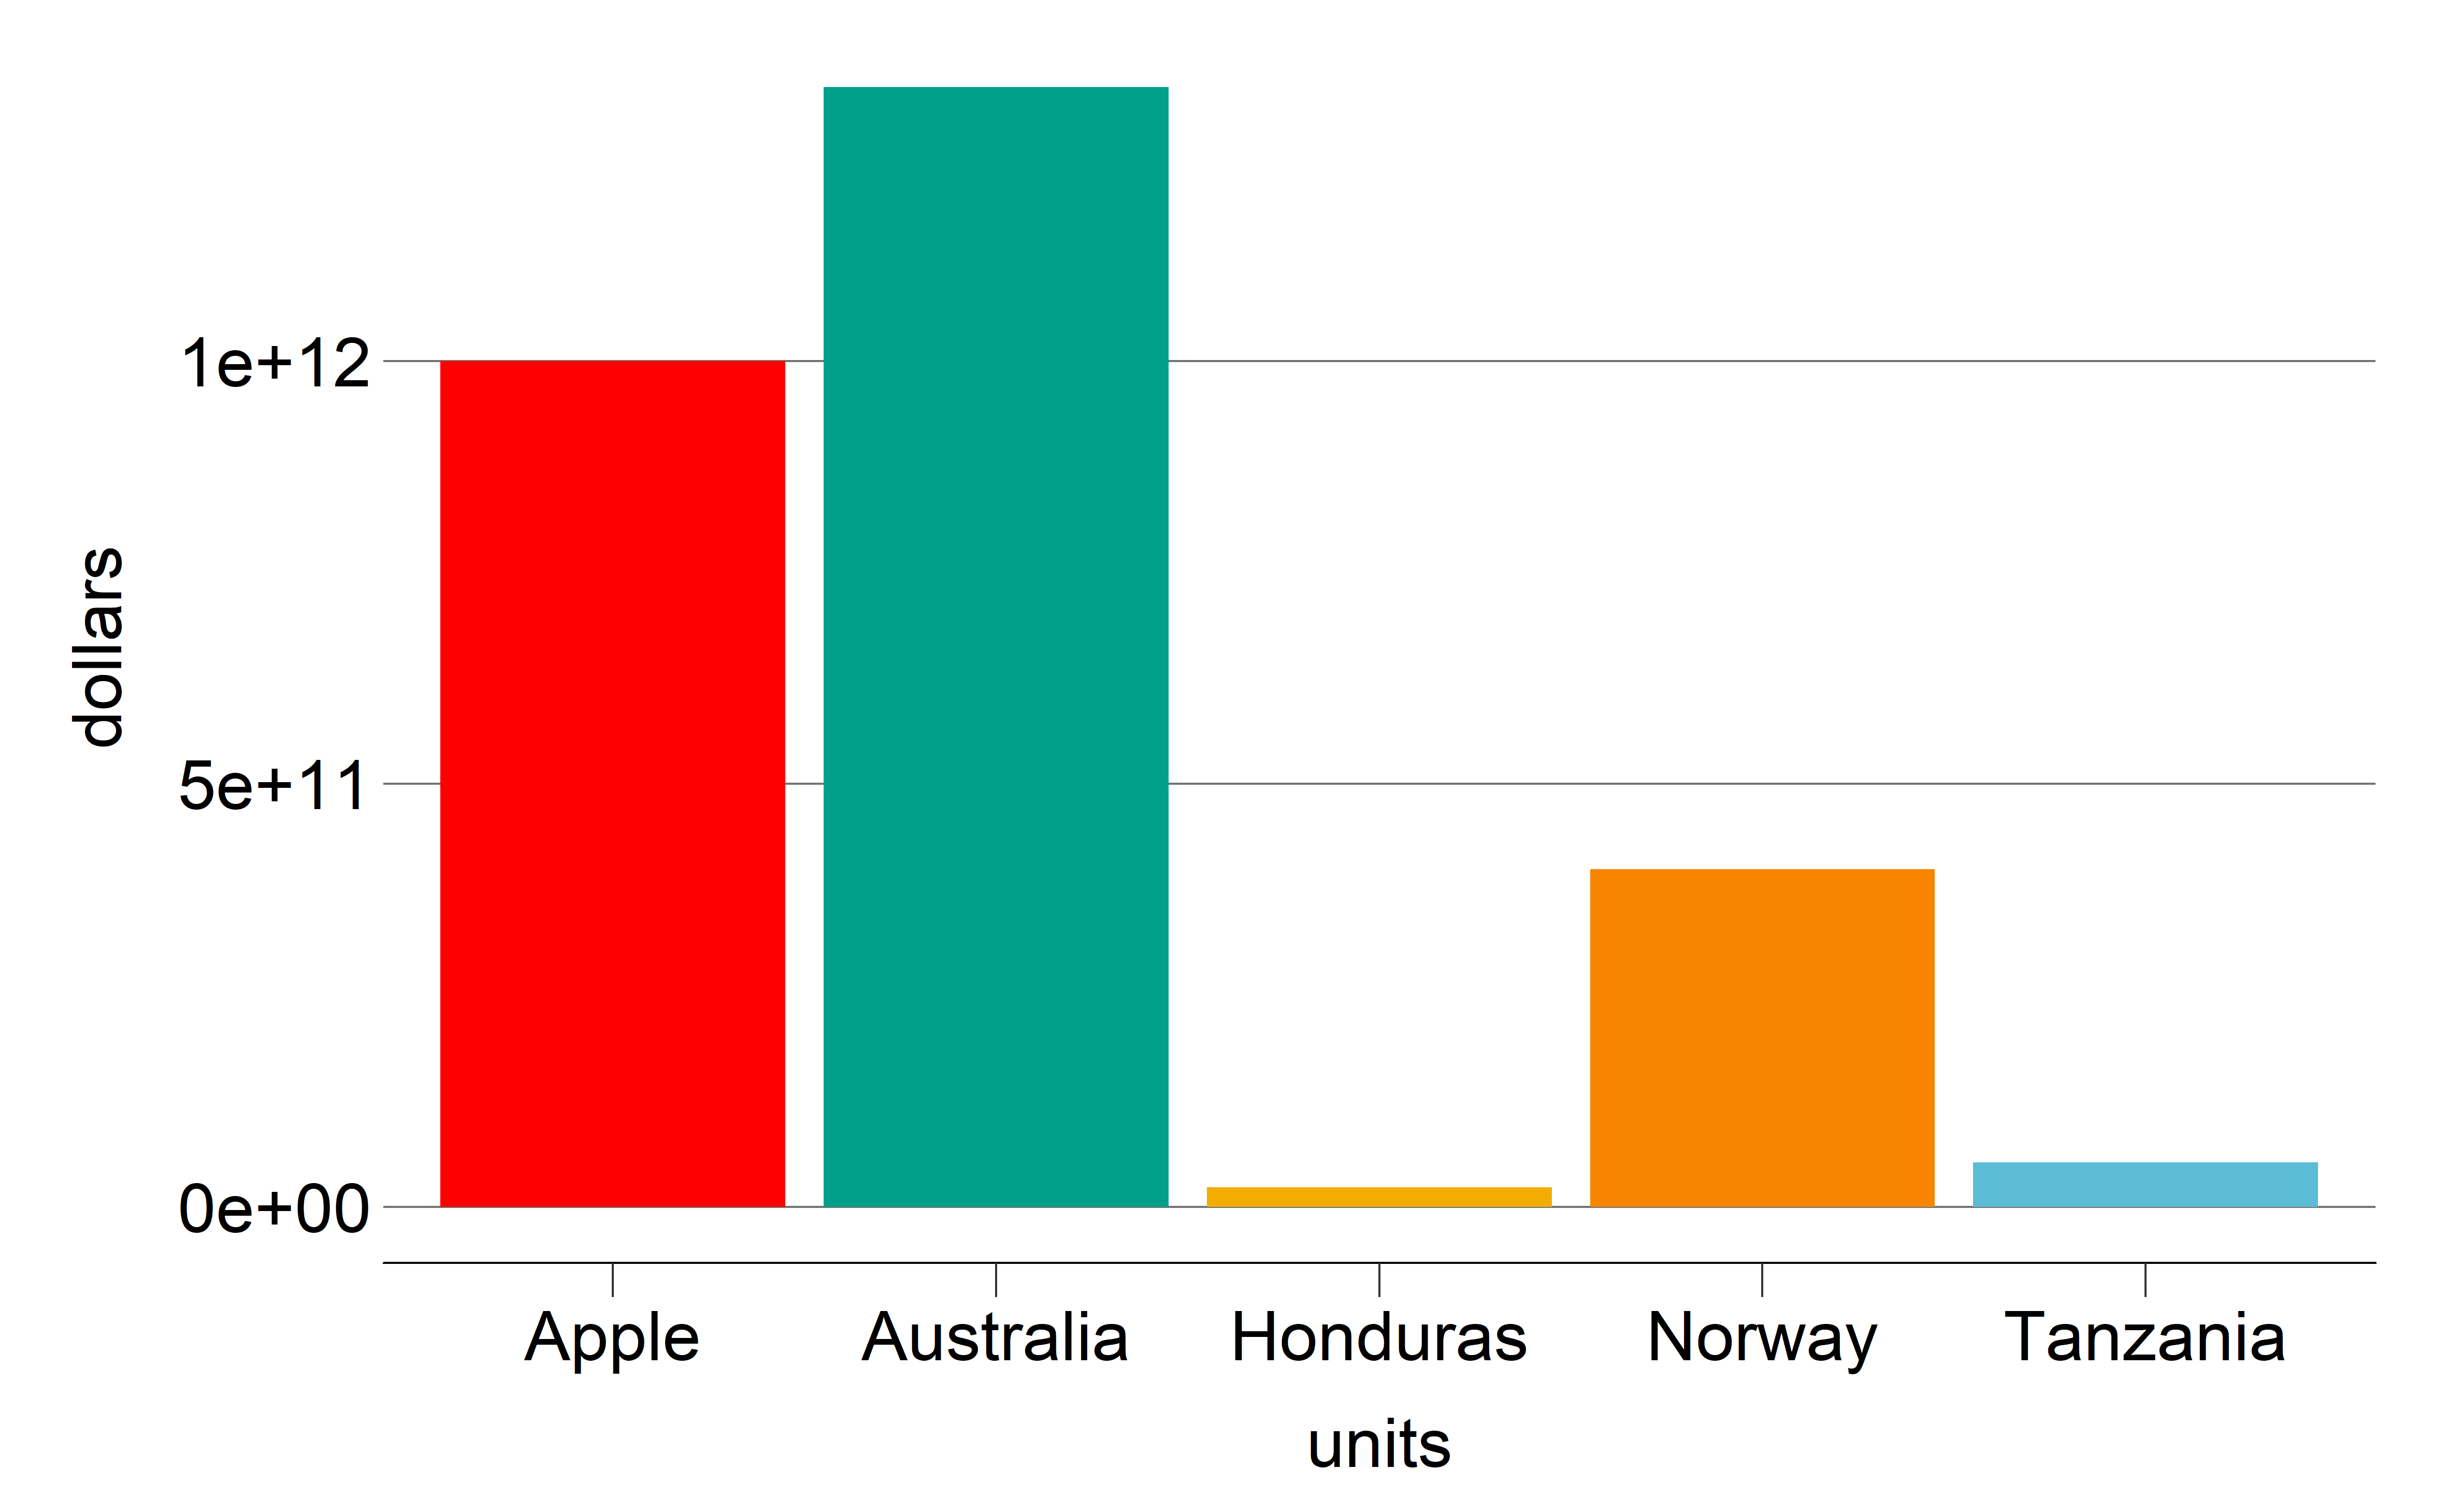
\includegraphics[width=\textwidth]{../img/value.png} % Comparing Aplles and ... States
    \label{fig:value}
\end{figure}
\end{frame}

\section{Keynesian Economics}
\begin{frame}{John Maynard Keynes (1883-1946)} 
    \begin{figure}
        \centering
        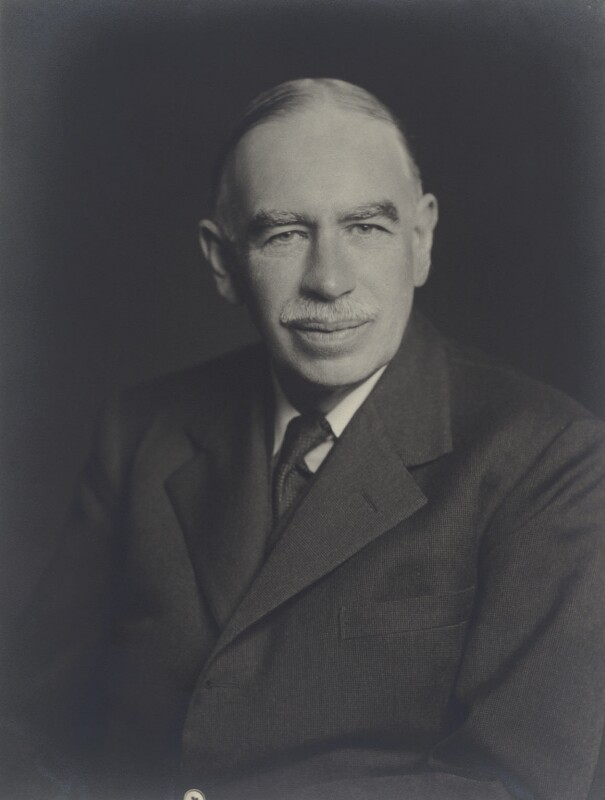
\includegraphics[width=0.5\textwidth]{../img/Lord_Keynes.jpg}
    \end{figure}{}
\end{frame}

\begin{frame}{The Great Depression}
        
       \begin{figure}[htpb]
       	\centering
       	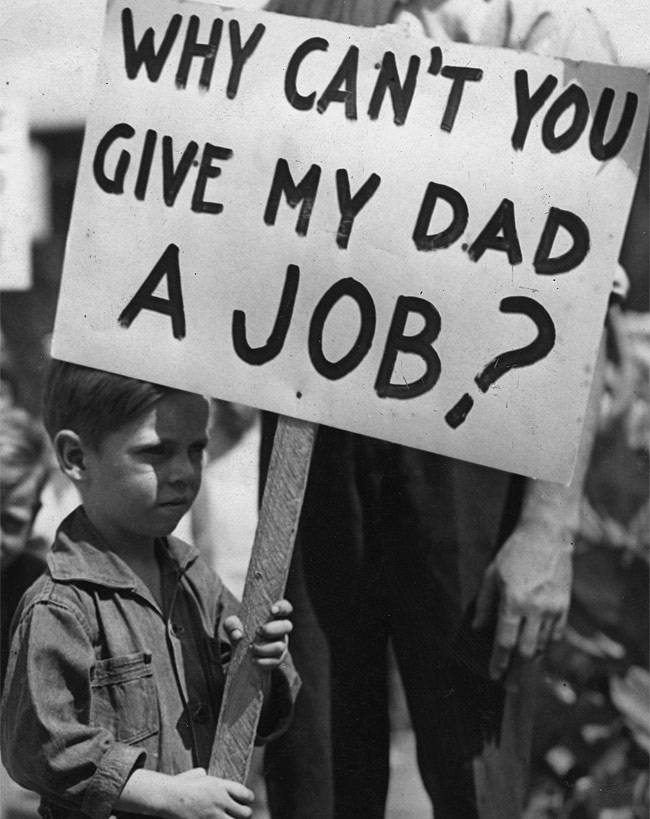
\includegraphics[width=0.6\linewidth]{../img/depression.jpeg}
       \end{figure} 
        
\end{frame}

\begin{frame}{Keynes' Solution}
\begin{itemize}
    \item $Y=C+I+G+X-M$ % Seminar stuff
    \item Step 1: Be the state
    \item Step 2: Increase aggregate demand % (Un)Employment is key
    
    
\end{itemize}
\end{frame}

\begin{frame}{``Pre-Keynesians"?}
\begin{itemize}
    \item FDR's New Deal
    \item Stalin
    \item "The true protagonist of the Keynesian ideas." - Galbraith (1977)
\end{itemize}
\end{frame}

\begin{frame}{Discussion}
     What would a neo-classical analysis of the Great Depression look like? % Unemployment -> wages dropping -> profits rising -> employers hire more workers -> unemployment is eliminated	- Unemployment as self-prescribed. - Stay out! Bust unions if necessary!
\end{frame}{}

\end{document} 

